\chapter{Introducción}\label{ch:introduccion}
\thispagestyle{empty}

\vspace{50pt}

\begin{adjustwidth}{50pt}{50pt}
    TODO
\end{adjustwidth}

\clearpage
\newpage
\thispagestyle{empty}
\mbox{}
\newpage

\cite{gutierrez2022, petavratzi2022, heredia2020, obaya2021, romero2021, fornillo2019}

Las otras aplicaciones de la Figura \ref{fig:iea-Li} incluyen dispositivos
electrónicos, medicamentos, lubricantes, entre otras \cite{IEA}.

\say{Sin embargo} el litio representa el 7 \% de la demanda de minerales críticos
para vehículos eléctricos mientras que para almacenamiento en la red el porcentaje
se encuentra en el 10 \%. El resto del porcentaje de la demanda está abarcado por 
otros metales y minerales críticos, tales como grafito, cobre, níquel, manganeso, 
cobalto y silicio \cite{IEA}.

\begin{figure}[h!]
    \centering
    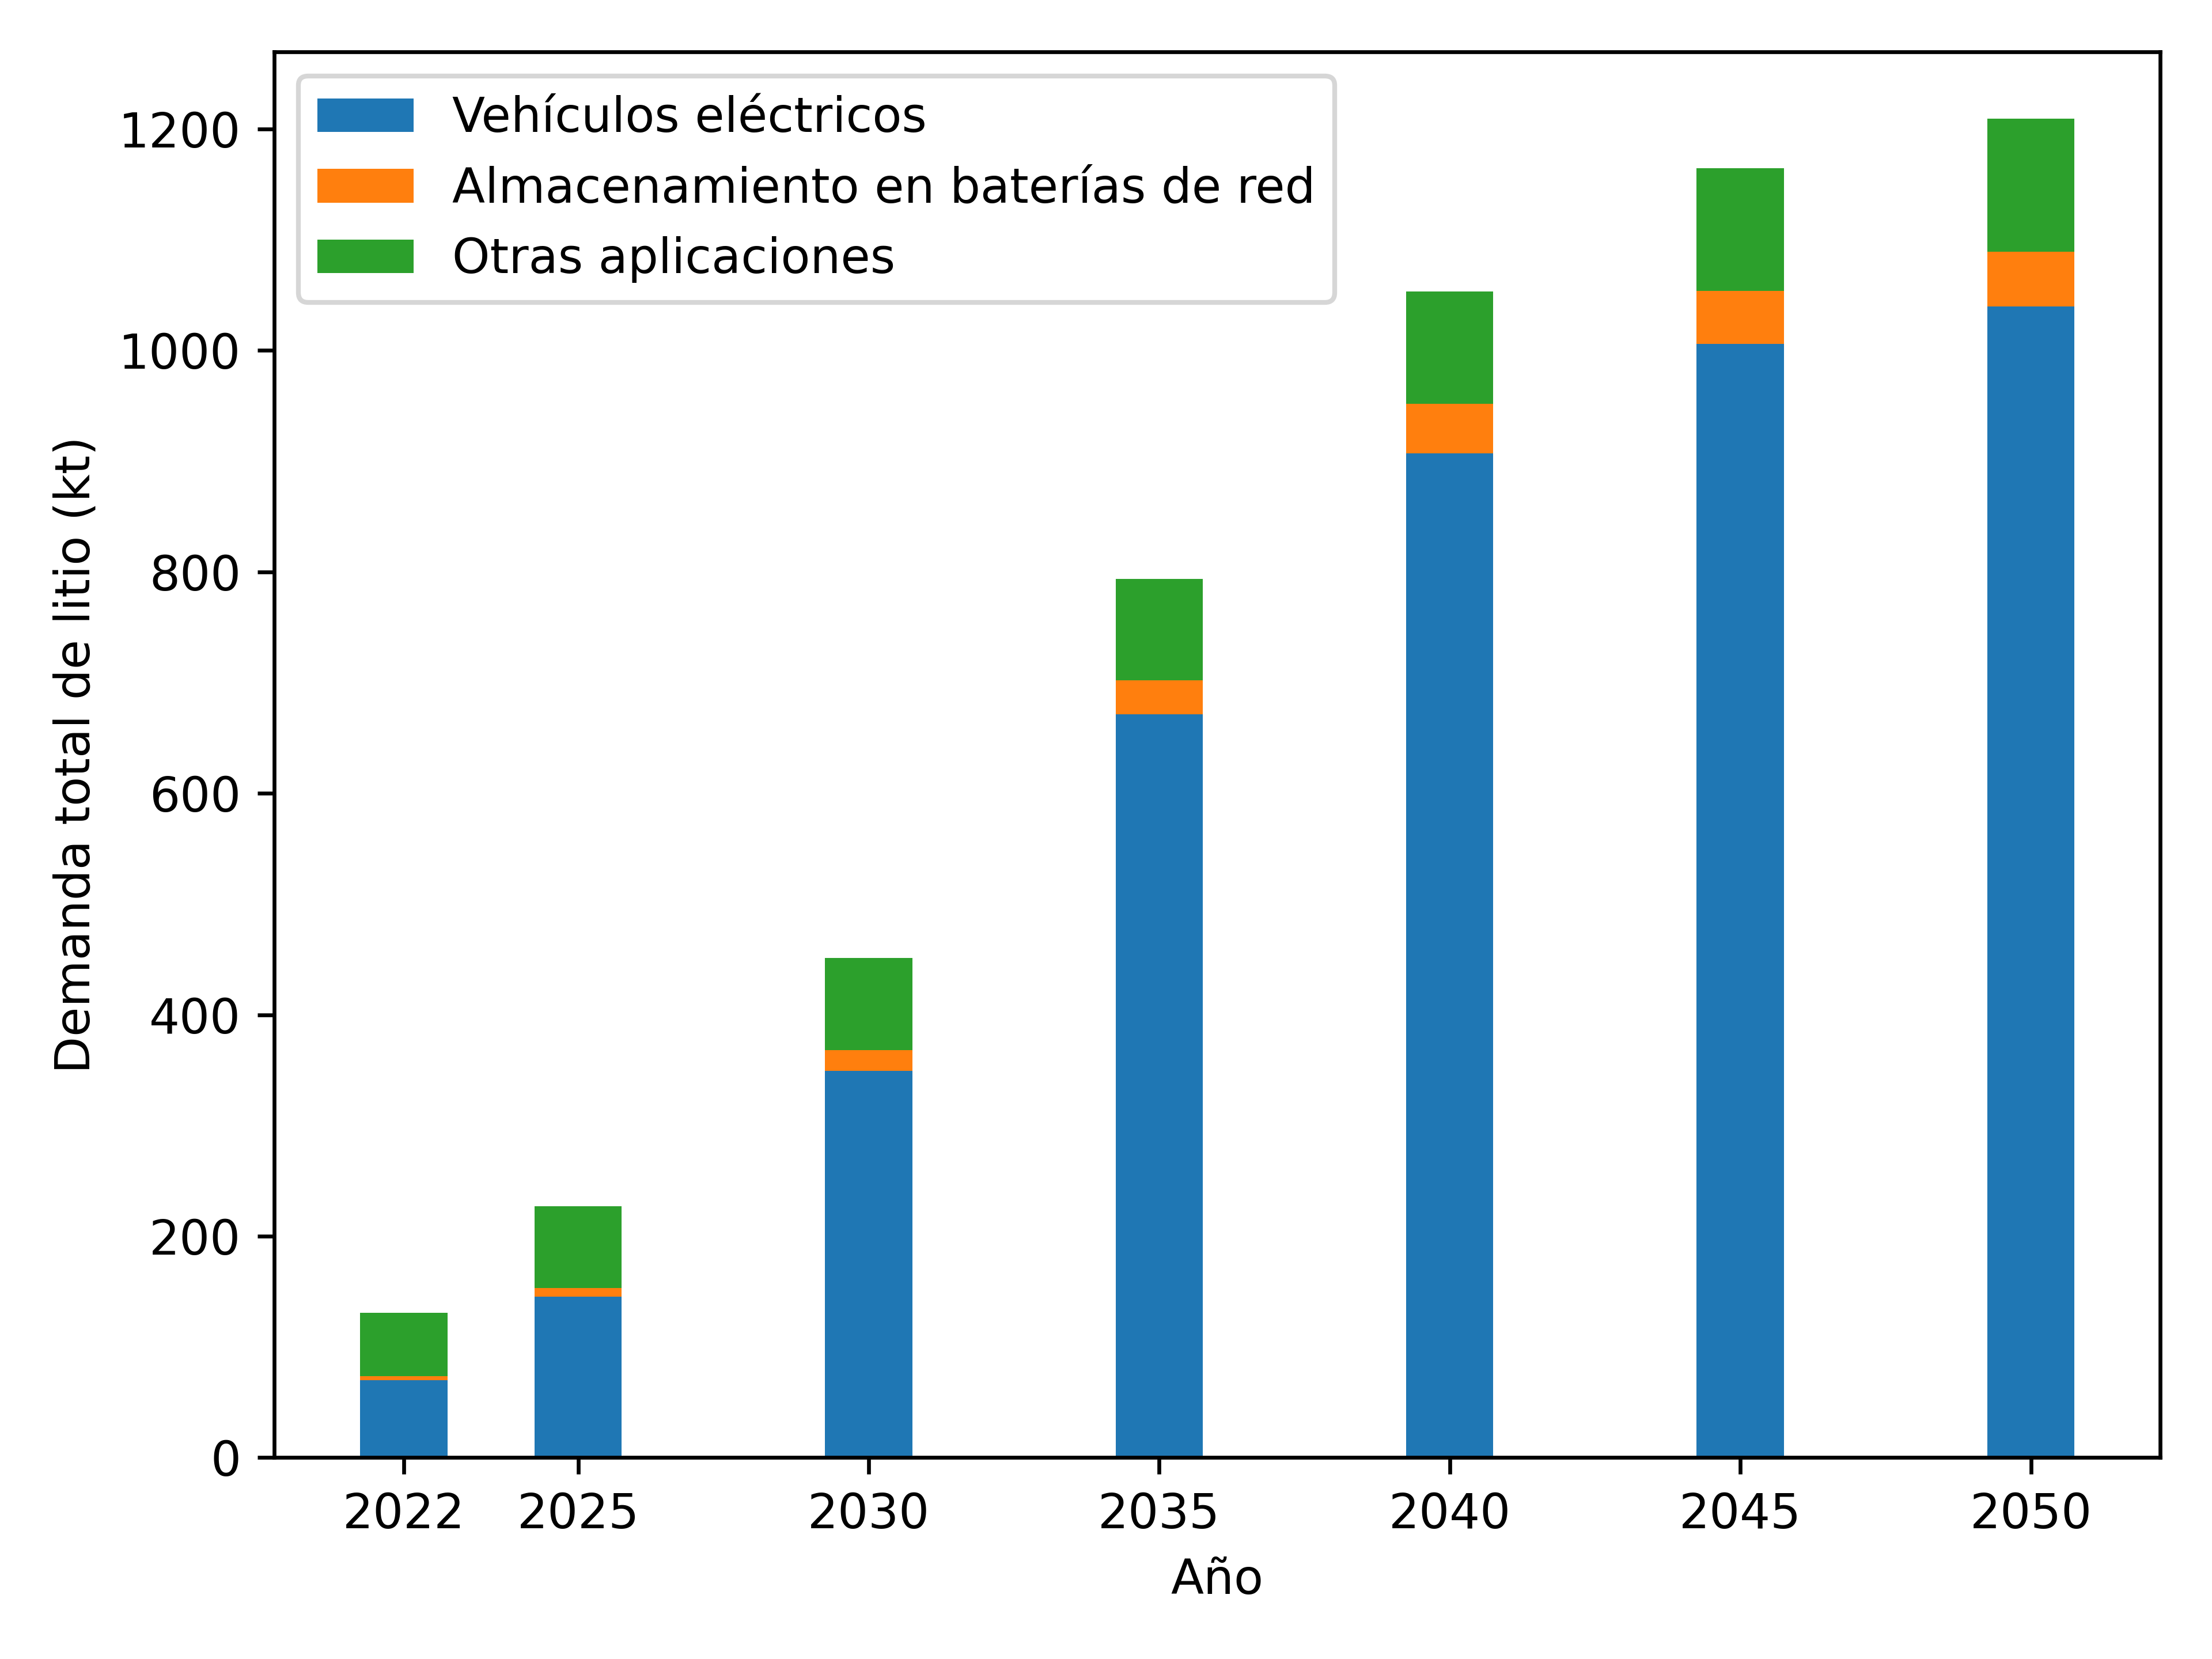
\includegraphics[width=.8\textwidth]{Introduccion/iea-Li.png}
    \caption{Proyección de la demanda total de litio en kilotoneladas por año y 
    aplicación. Fuente: \cite{IEA}.}
    \label{fig:iea-Li}
\end{figure}

\begin{figure}[h!]
    \centering
    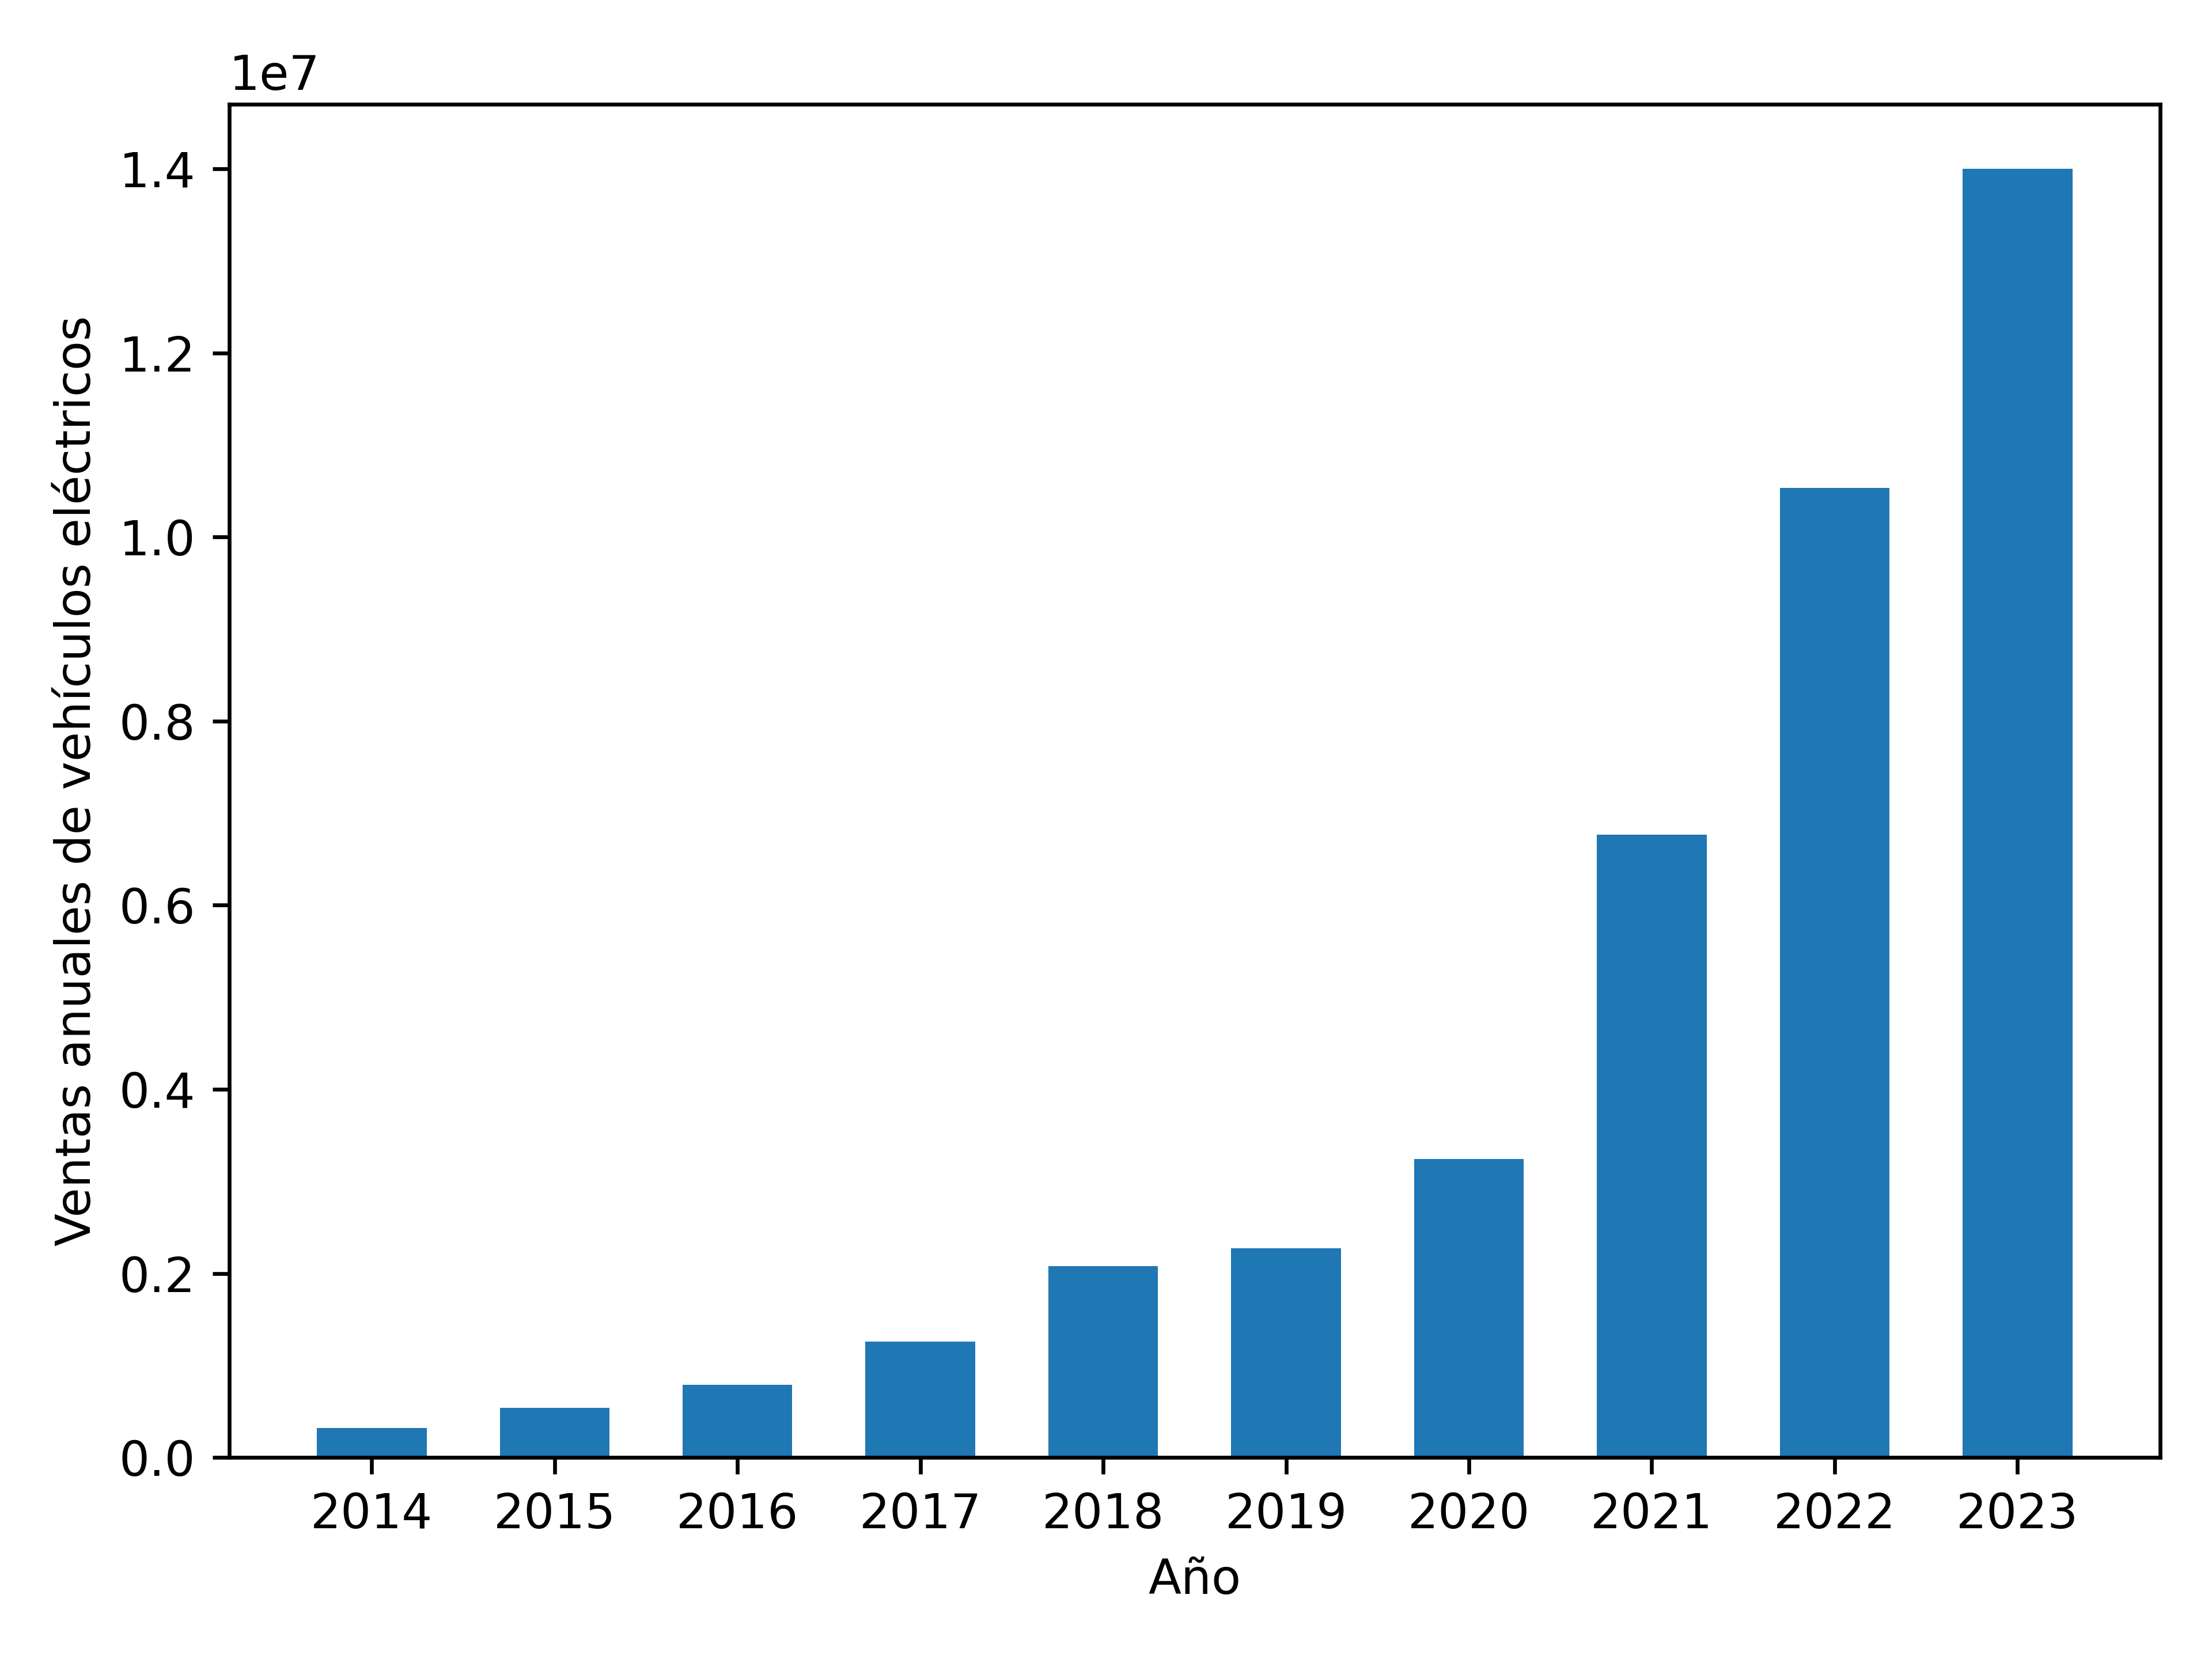
\includegraphics[width=.8\textwidth]{Introduccion/ev-volumes.png}
    \caption{Ventas anuales de vehículos eléctricos en la última década. Se 
    proyecta que para el 2030 las ventas asciendan a las 40 millones de unidades.
    Fuente: \cite{EVV}.}
    \label{fig:ev-volumes}
\end{figure}

\begin{figure}[h!]
    \centering
    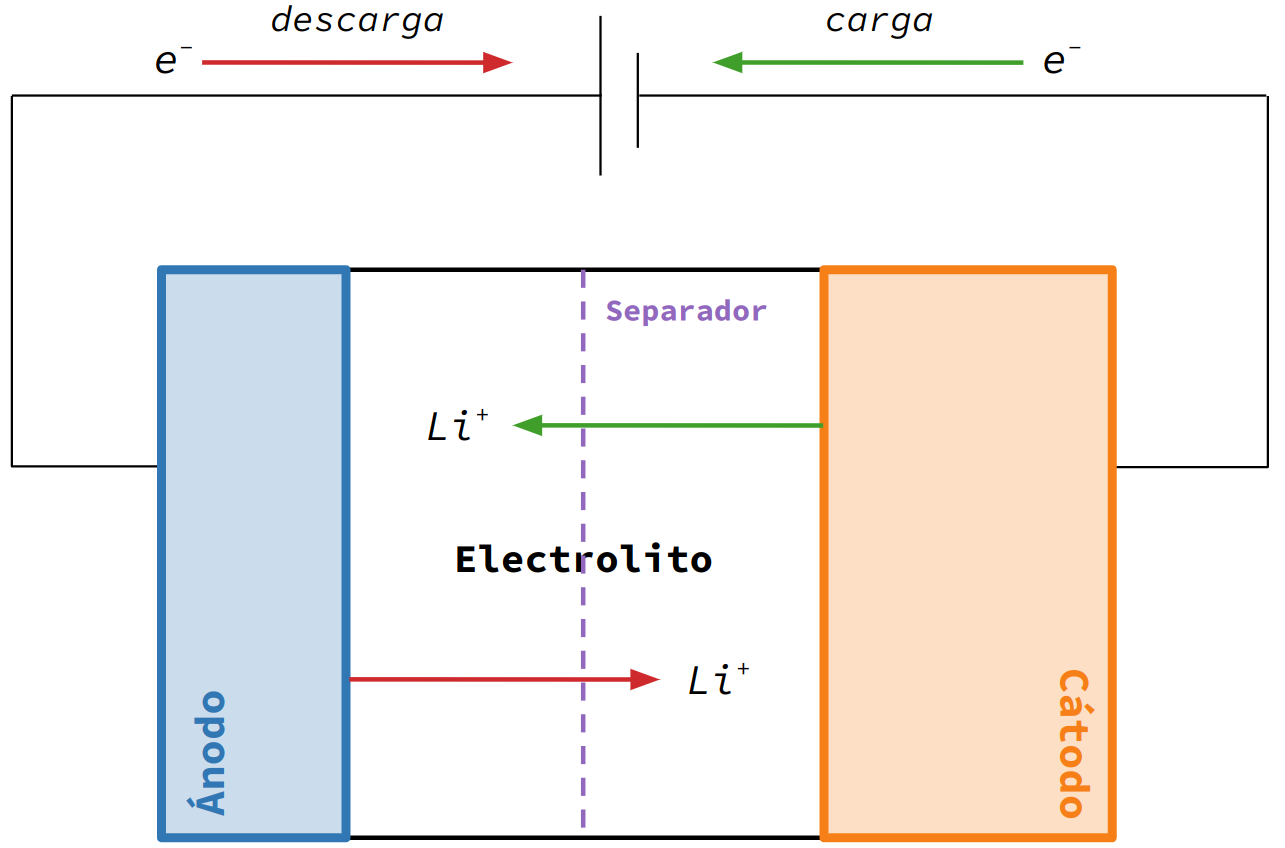
\includegraphics[width=.8\textwidth]{Introduccion/esquema_bateria.png}
    \caption{Esquema de las componentes y el funcionamiento de una batería de 
    ion-litio.}
    \label{fig:esquema-bateria}
\end{figure}
